\begin{filecontents*}{references.bib}
@article{nisan2006communication,
  author  = {Nisan, Noam and Segal, Ilya},
  title   = {The Communication Requirements of Efficient Allocations and Supporting Prices},
  journal = {Journal of Economic Theory},
  year    = {2006},
  volume  = {129},
  number  = {1},
  pages   = {192--224}
}

@inproceedings{lahaie2004applying,
  author    = {Lahaie, S{\'e}bastien M. and Parkes, David C.},
  title     = {Applying Learning Algorithms to Preference Elicitation},
  booktitle = {Proceedings of the 5th ACM Conference on Electronic Commerce},
  year      = {2004},
  pages     = {180--188}
}

@article{goldberg2020learning,
  author  = {Goldberg, Paul W. and Lock, Edwin and Marmolejo-Coss{\'i}o, Francisco},
  title   = {Learning Strong Substitutes Demand via Queries},
  journal = {ACM Transactions on Economics and Computation},
  year    = {2022},
  note    = {arXiv:2005.01496}
}

@incollection{parkes2006iterative,
  author    = {Parkes, David C.},
  title     = {Iterative Combinatorial Auctions},
  booktitle = {Combinatorial Auctions},
  editor    = {Cramton, Peter and Shoham, Yoav and Steinberg, Richard},
  publisher = {MIT Press},
  year      = {2006}
}

@inproceedings{parkes2000ibundle,
  author    = {Parkes, David C. and Ungar, Lyle H.},
  title     = {iBundle: An Efficient Ascending Price Bundle Auction},
  booktitle = {Proceedings of the 1st ACM Conference on Electronic Commerce},
  year      = {2000}
}

@misc{brero2019mlca,
  author        = {Brero, Gianluca and Lubin, Benjamin and Seuken, Sven},
  title         = {Machine Learning-powered Iterative Combinatorial Auctions},
  year          = {2019},
  eprint        = {1911.08042},
  archivePrefix = {arXiv},
  primaryClass  = {cs.GT}
}

@misc{lubin2020imlca,
  author        = {Lubin, Benjamin and Seuken, Sven and Beyeler, Manuel and Brero, Gianluca},
  title         = {iMLCA: Machine Learning-powered Iterative Combinatorial Auctions with Interval Bidding},
  year          = {2020},
  eprint        = {2009.13605},
  archivePrefix = {arXiv},
  primaryClass  = {cs.GT}
}

@misc{soumalias2023mlcca,
  author        = {Soumalias, Ermis and Weissteiner, Jakob and Heiss, Jakob and Seuken, Sven},
  title         = {Machine Learning-Powered Combinatorial Clock Auction},
  year          = {2023},
  eprint        = {2308.10226},
  archivePrefix = {arXiv},
  primaryClass  = {cs.GT}
}

@misc{soumalias2024mlhca,
  author        = {Soumalias, Ermis and Heiss, Jakob and Weissteiner, Jakob},
  title         = {Prices, Bids, Values: One ML-Powered Combinatorial Auction to Rule Them All},
  year          = {2024},
  eprint        = {2411.09355},
  archivePrefix = {arXiv},
  primaryClass  = {cs.GT}
}

@misc{huang2025llmproxies,
  author        = {Huang, David and Marmolejo-Coss{\'i}o, Francisco and Lock, Edwin and Parkes, David C.},
  title         = {Accelerated Preference Elicitation with LLM-Based Proxies},
  year          = {2025},
  eprint        = {2501.14625},
  archivePrefix = {arXiv},
  primaryClass  = {cs.GT}
}

@misc{soumalias2025llmassignment,
  author        = {Soumalias, Ermis and Jiang, Yanchen and Zhu, Kehang and Curry, Michael and Seuken, Sven and Parkes, David C.},
  title         = {LLM-Powered Preference Elicitation in Combinatorial Assignment},
  year          = {2025},
  eprint        = {2502.10308},
  archivePrefix = {arXiv},
  primaryClass  = {cs.AI}
}
\end{filecontents*}

\documentclass[11pt,a4paper]{article}

\usepackage[margin=1in]{geometry}
\usepackage{amsmath,amssymb,amsthm}
\usepackage{booktabs}
\usepackage{array}
\usepackage{enumitem}
\usepackage{xcolor}
\usepackage{microtype}
\usepackage{natbib}
\usepackage{longtable}
\usepackage{graphicx}
\usepackage{algorithm}
\usepackage{algpseudocode}
\usepackage{hyperref}

\hypersetup{colorlinks=true,linkcolor=blue,citecolor=blue,urlcolor=blue}

\newcommand{\G}{G}
\newcommand{\N}{N}
\newcommand{\B}{\mathcal{B}}
\newcommand{\C}{\mathcal{C}}
\newcommand{\E}{\mathcal{E}}
\newcommand{\X}{\mathcal{X}}
\newcommand{\K}{\mathcal{K}}
\newcommand{\V}{\mathcal{V}}
\newcommand{\R}{\mathbb{R}}
\newcommand{\argmax}{\operatorname*{arg\,max}}
\newcommand{\WDP}{\operatorname{WDP}}
\newcommand{\VCG}{\operatorname{VCG}}
\newcommand{\IM}{\operatorname{IM}}
\newcommand{\PV}{\operatorname{PV}}

\title{LLM Proxy-Assisted Combinatorial Auctions\\
\large A Modular Elicitation-Event Framework and Empirical Evaluation}
\author{Matthew Targett\\ \small MSc Computational Finance}
\date{\today}

\begin{document}
\maketitle

\begin{abstract}
Combinatorial auctions allow bidders to express values for packages of goods,
but their formal bid language and exponential bundle space can make
participation cognitively and technically demanding. This paper develops a
modular framework in which a person describes preferences in natural
language, an LLM-based proxy constructs an initial combinatorial bid, and the
auction mechanism emits elicitation events that identify economically salient
bundles for exact refinement. The framework separates environment generation,
preference interpretation, bid construction, mechanism feedback, and
evaluation, and is instantiated in iterative sealed and ascending clock
auctions. In 95 matched PC-component auction cases, interest-guided candidate
generation reduces the number of initially considered bundle values by 55.5\%
relative to full powerset support. Mechanism-driven refinement raises mean
allocation efficiency from 86.4\% to 94.8\% in the sealed format and 92.8\%
in the clock format, with the clock using fewer exact value queries. Payment
reconstruction remains less accurate than allocation recovery. The results
show how natural-language proxy assistance and mechanism feedback can be
combined in a reproducible auction architecture, while also identifying the
information that sparse elicitation leaves unresolved.
\end{abstract}

\noindent\textbf{Keywords:} combinatorial auctions; preference elicitation; large language models; proxy bidders; XOR bids; VCG; clock auctions; sealed auctions.

\section{Introduction}

Combinatorial auctions allocate heterogeneous goods when values depend on
packages rather than isolated items. They can express complements,
substitutes, and alternative configurations, but that expressiveness creates
two barriers to participation. First, \(m\) goods induce \(2^m\) possible
bundles. Second, bidders must translate informal preferences into a formal bid
language and reason about package values. Even where computation is available,
this reporting task can impose substantial cognitive and technical burden.

LLM-based proxies offer a possible interface between a person and that formal
market. A bidder can communicate in ordinary language, while a proxy interprets
the disclosure, constructs a combinatorial bid, and responds to structured
feedback \citep{huang2025llmproxies}. Such assistance could make expressive
auctions accessible to participants who would otherwise struggle to formulate
XOR package bids. This paper does not conduct a human-subject study and
therefore does not claim measured reductions in cognitive burden. Instead, it
develops and tests the computational architecture required for that interface.

The central proposal is an \emph{elicitation-event framework}. A proxy first
converts natural-language evidence into a structured interest map and an
initial set of provisionally valued bundles. During the auction, the mechanism
emits events that expose allocation-relevant or payment-relevant uncertainty.
The proxy maps each eligible event to a formal refinement action. This makes
the mechanism an elicitation environment rather than merely a passive consumer
of a one-shot LLM bid. The organising information path is
\[
\underbrace{\text{support discovery}}_{\text{what bundles are considered}}
\;\longrightarrow\;
\underbrace{\text{value estimation}}_{\text{how they are initially ranked}}
\;\longrightarrow\;
\underbrace{\text{mechanism-driven refinement}}_{\text{which estimates are corrected}}.
\]

Two contrasting mechanism families are evaluated:
\begin{enumerate}[leftmargin=*]
    \item an \textbf{iterative sealed XOR auction} with provisional feedback and final VCG payments;
    \item an \textbf{ascending clock mechanism} with supplementary XOR atoms and final VCG payments.
\end{enumerate}
They share the same initial proxy state and formal bid representation but
expose different evidence. The sealed mechanism repeatedly reveals provisional
allocations and counterfactual competitors. The clock produces a price and
demand trajectory that restricts the terminal verification frontier. Studying
both formats tests whether the event abstraction can accommodate distinct
mechanism-specific routes to economically salient bundles.

The event interface is designed to be extensible to other mechanisms, but
the empirical evidence is narrower: it covers two implemented mechanism
families, one generated PC-component master population, and one frozen model
configuration. The paper therefore distinguishes architectural generality
from empirical generalisation throughout.

The main research question is:
\begin{quote}
How can an LLM proxy translate natural-language preferences into a tractable
combinatorial bid, and how effectively can mechanism-specific elicitation
events refine that bid toward efficient allocation?
\end{quote}

The primary contribution is the modular elicitation-event interface. Three
supporting contributions make that interface testable and operational:
\begin{enumerate}[leftmargin=*]
    \item \textbf{A modular elicitation-event interface.} Sealed and clock mechanisms expose different economic signals through a common event abstraction, allowing targeted, deduplicated refinements and paired evaluation from the same frozen initial state.
    \item \textbf{Interest-guided candidate support and provisional initialisation.} A person-specific interest map determines what the proxy considers; provisional values then rank that support. This separates omission from scoring error.
    \item \textbf{Structured test environments.} A constrained pipeline produces heterogeneous private preferences and deterministic full-information benchmarks for auditable evaluation.
    \item \textbf{Information-aware diagnostics.} Candidate coverage, allocation trajectories, event incidence, and VCG witness logging identify whether information is lost during support selection, provisional scoring, allocation refinement, or payment-counterfactual construction.
\end{enumerate}

Caching, chunked structured output, fail-closed parsing, frozen replay, and
detailed provenance are supporting experimental controls rather than
independent conceptual contributions.

\section{Background and Literature Review}

This project lies at the intersection of classical preference elicitation, iterative and clock combinatorial auctions, machine-learning-powered elicitation, and recent work on LLM-based proxies.

\subsection{Classical Preference Elicitation}

Combinatorial auctions are appropriate when bidders have complements or substitutes across goods. Their central obstacle is communication. Nisan and Segal show that, for general valuation classes, efficient allocation can require exponential communication \citep{nisan2006communication}. This result motivates restricted bid languages, structured valuation classes, approximation, and selective elicitation.

Lahaie and Parkes connect preference elicitation to computational learning theory. They show how value queries can simulate membership queries and how certain demand-style queries can play the role of equivalence-query counterexamples \citep{lahaie2004applying}. This gives formal query-complexity guarantees for some structured valuation classes and bid languages, but it still assumes that bidders can answer formal economic queries. In practice, value and demand queries may be cognitively demanding.

Work on structured classes such as strong substitutes illustrates the same tension. Goldberg, Lock, and Marmolejo-Cossío study learning strong-substitutes demand via queries and show efficient algorithms for restricted settings but hard lower bounds in more general cases \citep{goldberg2020learning}. The theoretical lesson is that structure matters. The practical question is how to extract useful structure from human preference descriptions without requiring full formal revelation.

\subsection{Iterative and Clock Auction Design}

Iterative combinatorial auctions reduce upfront communication by eliciting information over rounds. Parkes surveys mechanisms that alternate between provisional allocations, price updates, and new bids \citep{parkes2006iterative}. iBundle is an early ascending package auction in which prices and provisional allocations guide bidders towards welfare-relevant packages \citep{parkes2000ibundle}. Such mechanisms motivate the iterative sealed arm in this project: each round solves a provisional WDP and uses the result to select bundles for refinement.

Clock auctions provide a different information structure. They post item prices, ask bidders for demanded bundles, and raise prices on over-demanded goods. In a clock setting, the proxy observes a price path and a sequence of revealed demands rather than only provisional winners and losers. These revealed bundles can subsequently delimit a sparse supplementary and counterfactual verification frontier.

The clock mechanism in this paper is CCA-inspired but not a full production CCA. It uses ascending item prices, top-surplus demand, accumulated supplementary XOR atoms, and final VCG payments. It does not implement activity-constrained supplementary bidding, optimised price increments, or core-selecting payments. This is intentional: the clock is used as a price-discovery environment whose revealed-demand path restricts later exact verification.

\subsection{Machine-Learning-Powered Elicitation}

Machine-learning-powered combinatorial auctions use partial bidder responses to train surrogate valuation models and select future queries. MLCA uses machine learning to guide value-query selection and reports high efficiency with comparatively few elicited values \citep{brero2019mlca}. iMLCA extends this idea by allowing interval bids and activity rules to reduce the reporting burden associated with exact values \citep{lubin2020imlca}.

More recent ML-powered clock mechanisms emphasise demand queries. Soumalias et al. propose an ML-powered combinatorial clock auction that learns from demand-query information and selects queries with high clearing potential \citep{soumalias2023mlcca}. Later work combines prices, bids, and values in a hybrid auction design \citep{soumalias2024mlhca}. This literature establishes welfare-versus-query-cost evaluation as a natural empirical standard and shows that query type matters. The present project differs by replacing direct human interaction with a proxy-mediated natural-language interface.

\subsection{LLM-Based Proxies}

Huang et al. propose LLM-based proxies for accelerated preference elicitation in combinatorial auctions \citep{huang2025llmproxies}. Their proxies interact with a mechanism on behalf of a bidder, maintain internal state, and use natural-language questions, value queries, demand queries, and learned bid representations. This is the closest conceptual predecessor to the present work. It motivates the distinction between a person model and a proxy model, and it demonstrates that LLMs can reduce the burden of translating qualitative preferences into formal bids.

Soumalias et al. study LLM-powered preference elicitation in combinatorial assignment \citep{soumalias2025llmassignment}. Their work similarly highlights the importance of protocol design, query cost, and LLM response variability.

The gap addressed here is mechanism portability. Existing LLM-proxy work is largely mechanism-specific. This paper asks how one event-driven proxy architecture behaves when embedded in sealed and clock mechanisms that expose different feedback signals.

\section{Formal Framework}

\subsection{Combinatorial Auctions and XOR Bids}

Let \(G=\{g_1,\ldots,g_m\}\) be a finite set of indivisible goods, and let \(\mathcal{B}=2^G\) be the bundle space. There are bidders \(N=\{1,\ldots,n\}\). Bidder \(i\) has a hidden valuation \(v_i:\mathcal{B}\to\mathbb{R}_{\geq 0}\). An allocation is \(a=(a_1,\ldots,a_n)\), where \(a_i\subseteq G\), subject to feasibility:
\[
a_i\cap a_j=\emptyset \quad \forall i\neq j.
\]
The full-information efficient allocation is
\[
a^* \in \argmax_a \sum_{i\in N} v_i(a_i).
\]

The implementation represents formal bids using XOR atoms. An XOR bid for bidder \(i\) is a finite set
\[
\theta_i=\{(b,\hat v_i(b)): b\in B_i\},
\]
where \(B_i\subseteq 2^G\). The induced reported valuation is
\[
v^{\theta_i}(b)=
\max_{\substack{b'\in B_i\\b'\subseteq b}}
\hat v_i(b'),
\]
with value zero if no reported atom is contained in \(b\). This free-disposal interpretation is used by the WDP solver.

Given reported bids \(\theta=(\theta_1,\ldots,\theta_n)\), the WDP is
\[
\max_a \sum_i v^{\theta_i}(a_i)
\]
subject to feasibility. The implementation solves this problem by an integer linear programming formulation over XOR atoms.

\subsection{Auction Environment and Person Model}

An auction environment is
\[
\mathcal{E}=(G,N,D_A,D_G,(\Lambda_i)_{i\in N},(v_i)_{i\in N}),
\]
where \(D_A\) is the auction description, \(D_G\) maps goods to public text
descriptions, \(\Lambda_i\) is bidder \(i\)'s private structured preference
profile, and \(v_i\) is the deterministic hidden benchmark valuation induced
by that profile. The bidder proxy observes the public catalogue and the
person's disclosed answer, but never observes \(\Lambda_i\) or \(v_i\). The
person simulator and evaluator may access the private profile for different
purposes.

The person simulator is distinct from the bidder proxy. Before an experiment,
the profile is rendered deterministically into a brief qualitative disclosure
contract \(D_i\). A person model conditioned on \(D_i\) answers one canonical
opening question, disclosing natural-language goals, positively valued
options, relevant alternatives or complements, acquisition mode, explicit
exclusions, and an approximate total budget. The answer is independently
verified against \(\Lambda_i\) before it is accepted.

During the principal mechanism runs, a value query for bundle \(b\) is
answered deterministically as \(v_i(b)\). This removes repeated LLM response
noise and isolates the bundle-selection policy induced by the auction
mechanism. LLM-based value and demand answers remain available as robustness
treatments, but they are not used in the main scalability specification.

The implementation records three model roles separately: environment,
person, and bidder proxy. The environment and person roles may use the same
model, while the bidder proxy can use a different provider and model. In the
current frozen population the environment and person roles use
\texttt{gpt-5.6-sol}, while interest-map and provisional-valuation inference
use \texttt{gemini-3.6-flash}. Role separation is an information boundary,
not necessarily a requirement that all roles use different model families.

\subsection{Structured Environment Generation}

The environment pipeline begins from a human-specified population design,
not an unconstrained request for an auction. The design fixes the 16 good
identifiers and descriptions, their functional categories, 16 bidder
archetypes across four broad strata, and population- and sample-level
constraints. It deliberately leaves bidder-specific numeric and structural
preferences to the environment model.

Each bidder is generated from a latent profile
\[
\Lambda_i=(w_i,\mathcal{S}_i,\mathcal{C}_i,B_i,\rho_i,D_i),
\]
where \(w_i\) gives base item values, \(\mathcal{S}_i\) person-specific
substitute groups, \(\mathcal{C}_i\) complement groups, \(B_i\) a budget cap
and scale, \(\rho_i\) saturation behaviour, and \(D_i\) a role and identity
description. Every good is also classified as core, secondary, low interest,
or zero value for that bidder.

For a substitute group \(S\in\mathcal{S}_i\), the profile gives full value to the highest-valued selected item and discounted backup or resale value to additional selected items:
\[
\operatorname{sub}_i(S,b)=
w_i(g^*)+\lambda_{iS}\sum_{g\in (b\cap S)\setminus\{g^*\}} w_i(g),
\quad
g^*\in\argmax_{g\in b\cap S} w_i(g).
\]
A complement group \(C\in\mathcal{C}_i\) contributes a bonus
\(\alpha_{iC}\) when \(C\subseteq b\). For ordinary single-system buyers,
\(\lambda_{iS}=0\) implements a \texttt{choose\_one} relationship. For
resellers, integrators, or multi-machine buyers, a positive backup factor
implements \texttt{can\_use\_multiple}. Thus functional similarity does not
imply that joint ownership is valueless. The generated value is a sum of
ordinary item contributions, substitute-group contributions, complement
bonuses, and saturation or cap adjustments. Values are repaired to satisfy
free disposal.

The environment model generates the structured profile rather than directly
enumerating a value for every bundle. Deterministic code then stores complete
hidden values for every non-empty bundle. For \(m\) goods this gives
\(2^m-1\) benchmark values per bidder. These tables support full-information
allocation, exact value queries, welfare evaluation, and diagnostic
decomposition.

Generation proceeds in batches with bounded automatic repair. A batch is
accepted only if its profiles satisfy schema, classification, monetary, and
person-level interest-density constraints. The assembled population is then
validated for per-good positive and core bidder coverage, cross-stratum
competition, multiway substitute structure, complement prevalence, and
acquisition-mode consistency.

\subsection{Coverage-Stratified Environment Sampling}

Experiments use a fixed validated 16-by-16 master population but vary the
selected goods and bidders. For each seed, a deterministic
coverage-stratified search creates one nested ordering of all goods and one
nested ordering of all bidders. Prefixes of these latent orderings generate
the required sizes while the public scenario preserves catalogue declaration
order.

Every scalability composition is validated for minimum interest coverage,
positive value for each selected bidder, complement and substitute
prevalence, category and bidder-stratum diversity, at least two
full-information winners, and a bound on the largest winner's welfare share.
The five selected composition seeds produce distinct good sets, bidder sets,
and combined environments for every experimental cell. They are alternative
nested orderings of one master population, not independently generated
populations.

\subsection{Event-Driven Proxy State}

Bidder \(i\)'s proxy has state
\[
S_i=(K_i,I_i,\mathcal{C}_i,O_i,\tilde v_i,\theta_i),
\]
where \(K_i\) is the knowledge base, \(I_i\) the interest map, \(\mathcal{C}_i\) the candidate bundle support, \(O_i\) explicit observations, \(\tilde v_i\) provisional or refined value estimates, and \(\theta_i\) the mechanism-facing XOR bid.

An elicitation event is represented as
\[
e=(\tau,i,b,x,\rho),
\]
where \(\tau\) is the event type, \(i\) the target bidder, \(b\) an optional
target bundle, \(x\) the mechanism state that triggered the event, and
\(\rho\) its eligibility evidence or economic rationale. This representation
separates three operations:
\[
E_t=\operatorname{Emit}_M(x_t),\qquad
q_t=\operatorname{Select}_{\pi}(E_t,S_t),\qquad
S_{t+1}=\operatorname{Update}(S_t,q_t,y_t),
\]
where the mechanism emits eligible events, the event policy selects an action,
and the proxy updates its state after response \(y_t\). A policy may prioritise
or ignore emitted events without changing the auction implementation, while a
new mechanism can emit the same event type from different state evidence.

The proxy responds to elicitation events:
\[
\pi_i:\mathcal{E}_{event}\times S_i \to (\mathcal{A}_{proxy},S_i').
\]
As a general interface, events may trigger language interaction, structural
inference, value or demand refinement, bid submission, or no action. This
expressiveness should not be confused with the experimental instantiation in
this paper. Here the opening exchange, interest map, candidate support, and
provisional values are frozen before the auction. At auction time, a
deterministic event policy selects an unqueried bidder--bundle pair, exact
value lookup deterministically returns the hidden benchmark value, and that
value replaces the provisional report. The runner does not deliberate over a
transcript, autonomously choose a new query type, or make any auction-stage LLM
call. The proxy state therefore defines a reusable general architecture, while
the experiments evaluate a deliberately non-agentic event-policy
instantiation.

The generic update is
\[
e_t \to \pi_i(e_t,S_{i,t}) \to q^V_{i,t}(b) \to v_i(b)
\to S_{i,t+1} \to m_{i,t+1}.
\]
For sealed auctions, \(m_{i,t+1}\) is an XOR bid. For clock auctions, it is a demand response and supplementary XOR information.

\section{Proxy Inference Pipeline}

\subsection{Natural-Language Questioning}

The current main configuration uses one canonical opening question tailored
to the PC-component catalogue. It asks what the person hopes to obtain, how
the alternatives fit their needs, whether any goods are useful only together
or remain useful in multiples, and approximately how much they would spend
overall. The same question is used across bidders in a given catalogue so
that differences in their answers arise from preferences rather than
question wording.

The person answer is intentionally brief and qualitative. It is not intended
to recover a complete value table. It discloses enough information to support
candidate selection and approximate scale without exposing base values,
complement bonuses, or the hidden bundle table. The answer and its
preparation-time verification record are frozen before either auction
mechanism is run. Proxy-generated opening questions remain an optional
robustness treatment.

\subsection{Interest Map}

The proxy derives a lightweight interest map from the auction description, item descriptions, natural-language question, and person answer:
\[
I_i=(G_i^+,G_i^-,C_i,S_i,\beta_i,r_i).
\]
Here \(G_i^+\) is the inferred interested item set, \(G_i^-\) excluded items, \(C_i\) complement groups, \(S_i\) substitute groups, \(\beta_i\) a budget hint, and \(r_i\) a rationale.

Each inferred substitute group additionally records an acquisition mode
\[
\mu(S)\in
\{\texttt{choose\_one},\texttt{can\_use\_multiple},\texttt{unclear}\}
\]
and textual evidence. A restrictive \texttt{choose\_one} mode is accepted
only when the answer states that at most one member is useful or that
additional members add no meaningful value. Ranking one good above another,
calling an item a fallback, or observing functional similarity is
insufficient. This distinction prevents a GPU category, for example, from
being incorrectly treated as exclusive for a reseller who can use multiple
cards.

The main implementation uses a closed-world map: every catalogue item must
be classified, and an item that is neither positively disclosed nor included
in a disclosed structural group is placed in \(G_i^-\). Candidate generation
considers subsets of interested items, never includes excluded items, and
filters joint bundles only when they contain multiple members of an
evidence-grounded \texttt{choose\_one} group. \texttt{Can\_use\_multiple} and
\texttt{unclear} groups are retained conservatively.

The implementation enforces only generic consistency. It does not impose
hidden PC-build-specific rules or use the private profile to repair the
proxy's map. Hidden truth is used solely for diagnostics: item
precision/recall, exact group precision/recall, acquisition-mode accuracy,
choose-one precision/recall, dangerous false exclusivity, and
oracle-versus-inferred candidate-set precision and recall.

The current implementation also avoids silent full-powerset fallback in live experiments. If interest-map parsing fails after retries, the run can fail closed under an interest-map failure policy. A degraded all-items fallback remains available for debugging, but it is not the preferred experimental setting because it can generate excessively broad and incoherent support.

\subsection{Candidate Bundle Generation}

Given \(I_i\), candidate generation produces a priority-ordered set
\[
\mathcal{C}_i=\Psi(I_i,G,M_{\mathrm{cand}}).
\]
The implemented ordering is:
\begin{enumerate}[leftmargin=*]
    \item complete declared complement groups;
    \item singletons of interested items;
    \item all remaining valid subsets in ascending size and lexicographic order.
\end{enumerate}
A bundle is valid if it does not include multiple goods from the same
declared \texttt{choose\_one} substitute group. Bundles containing multiple
members of \texttt{can\_use\_multiple} or \texttt{unclear} groups remain
eligible. A candidate cap \(M_{\mathrm{cand}}\) can be applied after
prioritisation, although the principal scalability preparation uses
\(M_{\mathrm{cand}}=\infty\) and therefore leaves the inferred support
uncapped.

This design intentionally keeps the interest map simple. Its main function is to reduce support size while preserving important complement groups and singletons. Failure modes are logged through candidate-count diagnostics, candidate reduction ratios, coverage measures, and interest-map quality flags such as broad interest sets with no substitute groups.

\subsection{Provisional Valuation and Chunking}

After candidate generation, the proxy assigns provisional values:
\[
\tilde v_i(b),\quad b\in\mathcal{C}_i.
\]
The proxy model receives the public catalogue, opening exchange, interest
map, and enumerated candidate support. It returns one estimated value for
each candidate bundle. These values both rank the support and initialise the
proxy's mechanism-facing XOR bid. They are proxy-side inferences, not person
value queries, and they do not have access to the private profile or hidden
valuation table.

For large supports, the implementation uses deterministic PV chunking. If
\[
|\mathcal{C}_i|>K_{\PV},
\]
candidate bundles are split into ordered chunks of at most \(K_{\PV}\) bundles. Each chunk is valued by a separate provisional-valuation call and the results are merged. Chunking preserves the semantics of the initial bulk PV stage while reducing the risk of truncation or malformed large JSON outputs. PV chunks are counted as shared initial proxy inference calls, not value-query refinements.

The current preparation configuration uses chunks of at most 64 bundles and
fail-closed PV behaviour. If a chunk fails after parse retries, the run
aborts with a diagnostic error identifying the bidder, candidate count,
chunk size, token budget, and original parsing exception. A degraded
zero-initialisation policy exists for debugging, but failed PV never triggers
mass direct value queries over the candidate support. Otherwise a structured
output failure would silently change the elicitation treatment and
contaminate person-query counts.

\subsection{Provisional-Value Calibration}

Provisional valuations are estimated from the person's short qualitative
disclosure alone, and the estimator's error need not be centred. The
implementation therefore supports an explicit calibration of the raw
provisional value, parameterised by a family, a multiplicative scale, and an
optional bundle-size adjustment:
\[
\hat v^{cal}(b)=\min\Bigl\{\bar B,\;
  s\cdot \hat v^{raw}(b)\cdot \gamma^{\max(0,|b|-k_0)}\Bigr\}.
\]
Here \(s>0\) is the scale, \(\gamma>0\) the size factor, \(k_0\) the size
threshold, and \(\bar B\) the bidder's \emph{disclosed} budget, taken from the
elicited interest map rather than from any hidden value. The scale is not
restricted to \((0,1]\): the estimator's qualitative conservatism instructions
mean the observed bias is typically downward, so the corrective scale is
generally greater than one. The family selects which terms apply: the
identity (raw values), scale only, or scale with the size adjustment.

Calibration applies only to initial LLM-inferred provisional values. Exact
deterministic value-query answers and mechanism-triggered refinements are
ground truth and are reported unchanged.

Frozen elicitation packs store raw, uncalibrated provisional values, so
alternative calibration rules are replayed over an identical elicitation
without new LLM calls; a calibrated and an uncalibrated arm therefore differ
only in the calibration and not in re-elicitation noise. Every run records its
fully resolved effective calibration, together with a stable configuration
hash, in its console header, machine-readable run configuration, and result
tables.

The final specification uses the accepted uniform scale \(s=1.4758\), a
disclosed-budget cap, and no bundle-size adjustment (\(\gamma=1\)). It was
selected before the main mechanism runs using nine synthetic consumer-bundle
environments spanning camera/video, kitchen, and travel domains, with three
independently generated instances per domain. Three folds leave out one
instance index across all domains, fitting on six environments and evaluating
on the remaining three. The objective is mean absolute reported-VCG payment
error normalised by optimum welfare, subject to a mean-efficiency tolerance.
This procedure shares no goods or bidder profiles with the PC-component
population. On the nine held-out evaluations, calibration reduces the
objective from 0.289 to 0.233 and improves seven of nine cases. The accepted
calibration and its hash are frozen in the final experiment specification.

\begin{algorithm}[htbp]
\caption{Natural-language disclosure to initial XOR bid}
\label{alg:initial-bid}
\begin{algorithmic}[1]
\Require Public catalogue \(G\), canonical question, person disclosure contract \(D_i\)
\State Obtain and independently verify opening answer \(A_i\)
\State Infer interest map \(I_i\) from \((G,A_i)\)
\State Generate \(\mathcal C_i=\Psi(I_i,G,M_{\mathrm{cand}})\)
\State Estimate \(\tilde v_i(b)\) for every \(b\in\mathcal C_i\), using deterministic chunks if required
\State Apply the frozen calibration rule and disclosed-budget cap
\State \Return \(\theta_i^0=\{(b,\tilde v_i(b)):b\in\mathcal C_i\}\) and frozen proxy state \(S_i^0\)
\end{algorithmic}
\end{algorithm}

\subsection{Caching, Freezing, and Replay}

LLM calls are cached by a hash of the rendered prompt and all
response-relevant metadata. Cache modes include off, read-write, read-only,
and refresh. Each successful response is committed independently, allowing
interrupted preparation to resume without repeating completed calls.

Caching supports preparation, but the principal experimental control is the
frozen elicitation pack. A pack contains the accepted opening exchange,
interest map, candidate bundles, raw provisional values, model provenance,
generation settings, and call records for one catalogue and bidder set.
Fresh mutable proxies replay this immutable initial state with zero LLM calls.
Consequently sealed and clock arms differ only in their mechanism paths and
deterministic refinement queries.

Initial elicitation depends on the selected goods but not on the number of
rival bidders. For each seed, preparation therefore generates one master pack
for every goods count and then projects ordered bidder subsets into the 19
scalability cells. This avoids regenerating the same bidder-catalogue exchange
for the fixed-goods bidder sweep.

\section{Mechanism Environments}

\subsection{Iterative Sealed XOR Auction}

At round \(r\), each proxy submits an XOR bid \(\theta_i^r\), and the
mechanism solves:
\[
a^r\in\argmax_a\sum_i v^{\theta_i^r}(a_i).
\]
The WDP and reported allocation provide the mechanism state from which events
are emitted; the auction algorithm itself does not prescribe which bundle is
queried. After each set of event responses, corrected XOR atoms replace their
provisional counterparts and the WDP is solved again. The main termination
condition is the absence of any eligible new refinement after at least one
cycle. Forty rounds is a non-binding runaway safeguard in the final suite.
Every bidder--bundle query is deduplicated globally.

\subsection{Sealed Elicitation Events}

Four event families are considered because they expose different parts of the
reported allocation frontier.

\paragraph{Incumbent verification.}
The provisionally allocated bundle is the atom whose error can most directly
invalidate the reported winner. Whenever a bidder receives a non-empty,
previously unqueried bundle in the current WDP allocation, the event targets
that bidder--bundle pair for exact value lookup.

\paragraph{Winner-removal allocation counterfactual.}
VCG payments and competitive displacement depend on allocations that become
feasible when a current winner is absent. For each winning atom, the mechanism
temporarily removes that atom, re-solves the WDP, and emits events for
previously unqueried bundles that enter the counterfactual allocation.

\paragraph{Scarcity-avoiding fallback.}
A high provisional incumbent may occupy contested goods even when its bidder
has a credible alternative. If an incumbent contains currently contested
goods, the event selects the bidder's highest-reported unqueried alternative
that reduces contested-good exposure and retains at least 60\% of the
incumbent's reported value. It is triggered at most once per bidder.

\paragraph{Large-correction follow-up.}
A large initial error is evidence that a nearby provisional ranking may also
be unreliable. If exact lookup changes a value by at least 25\% under the
symmetric relative correction measure, the event targets one unqueried
structurally neighbouring candidate bundle. It is triggered at most once per
bidder.

Independent loser exploration is disabled in the principal experiments:
losers are queried only when they enter a winner-removal allocation. Section
\ref{sec:policy-ablation} selects among combinations of the four events; the
definitions above do not presuppose that every event is empirically useful.

\begin{algorithm}[htbp]
\caption{Iterative sealed elicitation}
\label{alg:sealed}
\begin{algorithmic}[1]
\Require Frozen initial bids \(\theta^0\), sealed event policy \(\pi_S\)
\For{round \(r=0,1,\ldots\)}
    \State Solve the reported WDP to obtain \(a^r\)
    \State \(E_r\gets\operatorname{Emit}_{S}(a^r,\theta^r)\)
    \State Remove previously queried bidder--bundle pairs from \(E_r\)
    \State \(Q_r\gets\operatorname{Select}_{\pi_S}(E_r,S^r)\)
    \If{\(Q_r=\emptyset\) after at least one elicitation cycle} \State \textbf{break} \EndIf
    \ForAll{\((i,b)\in Q_r\)} \State Replace \(\tilde v_i(b)\) by exact \(v_i(b)\) \EndFor
\EndFor
\State \Return final reported allocation and reported-space VCG payments
\end{algorithmic}
\end{algorithm}

\subsection{Ascending Clock with Supplementary XOR Bids}

The clock arm posts item prices \(p_t\). The reported surplus of bundle \(b\) for bidder \(i\) is
\[
u_{i,t}^{\theta}(b)=v^{\theta_{i,t}}(b)-\sum_{g\in b}p_{t,g}.
\]
Each proxy reports up to \(k\) top-surplus bundles; the principal
specification uses \(k=3\). The mechanism increments every good with positive
excess demand by \$50. All top-\(k\) demands observed along the price path are
accumulated as supplementary XOR atoms. No exact value query is made while
prices ascend: price discovery is therefore allowed to complete on the
frozen calibrated reports. The clock stops when there is no excess demand;
500 rounds is a runaway safeguard rather than a target.

Thus price discovery is query-free and naturally terminates before terminal
exact refinement begins. Let \(R_i\) denote bidder \(i\)'s bundles revealed
among its top-\(k\) demands. These revealed sets delimit the clock-specific
event space: unrevealed losing bundles do not become eligible merely because
they have high provisional values.

\subsection{Clock Elicitation Events}

\paragraph{Single-pass revealed VCG witness.}
Before any correction, the mechanism removes each provisional winner and
solves the associated supplementary counterfactual allocation. This freezes a
pre-query witness frontier. An event is emitted only when a counterfactual
bundle is both unqueried and belongs to its bidder's revealed-demand set
\(R_i\). The event targets payment-relevant competitors while preserving the
support discipline supplied by clock price discovery.

\paragraph{Winner closure.}
Corrections can change the supplementary allocation. After each re-solve, an
event is emitted for every newly allocated, previously unqueried bundle. The
mechanism alternates exact lookup and re-optimisation until all current winners
have been verified. This targets allocation correctness rather than broad
frontier exploration.

\paragraph{Staged revealed-witness closure.}
Winner corrections can expose new bidder-removal competitors. The mechanism
therefore recomputes the revealed witness frontier after winner closure,
queries eligible revealed witnesses, and returns to winner closure. The two
stages alternate until neither produces a new query. Section
\ref{sec:policy-ablation} evaluates this sequence against narrower and broader
terminal policies.

\begin{algorithm}[htbp]
\caption{Clock price discovery and terminal revealed-winner verification}
\label{alg:clock}
\begin{algorithmic}[1]
\Require Frozen bids \(\theta^0\), top-\(k\) rule, price increment \(\Delta p\)
\While{some good has positive excess demand}
    \State Record each bidder's top-\(k\) positive-surplus demands in \(R_i\)
    \State Raise each over-demanded good's price by \(\Delta p\)
\EndWhile
\State Construct supplementary XOR bids from all revealed demands
\State Freeze and query eligible pre-correction revealed VCG witnesses
\Repeat
    \State Query newly allocated unverified bundles until winner closure
    \State Recompute and query eligible revealed bidder-removal witnesses
\Until{neither stage emits an unqueried bidder--bundle pair}
\State \Return final supplementary allocation and reported-space VCG payments
\end{algorithmic}
\end{algorithm}

\subsection{Payments and the Information Required by VCG}

VCG is retained as a common reported-space payment rule so that sealed and
clock allocation paths remain comparable. Payment accuracy is analytically
distinct from allocation efficiency. Even if every finally allocated bundle
has been queried exactly and the efficient allocation has been found, bidder
\(i\)'s payment depends on the welfare attainable by the other bidders when
\(i\) is removed. Sparse provisional reports can therefore yield accurate
allocations but inaccurate winner-removal counterfactual welfare and revenue.

Allocation efficiency is consequently the primary mechanism outcome.
Reported VCG revenue, full-information VCG revenue, and per-winner payment
error are reported as secondary diagnostics. A post-allocation
payment-counterfactual audit is a natural extension, but replacing VCG with
pay-as-bid would conflate preference elicitation with strategic bid shading
and is not part of the principal design.

\begin{table}[ht]
\centering
\caption{Feedback signals by mechanism.}
\label{tab:mechanism-feedback}
\begin{tabular}{p{0.27\linewidth}p{0.32\linewidth}p{0.33\linewidth}}
\toprule
Mechanism & Main feedback & Proxy refinement opportunity \\
\midrule
Sealed XOR--VCG & Provisional WDP, allocated bundles, winner-removal frontier, contested goods & Refine current winners, counterfactuals, scarcity fallbacks, and one-step correction neighbours \\
Clock with supplementary VCG & Ascending prices, top-three revealed demands, terminal winner-removal frontier & After price discovery, close newly winning bundles and revealed VCG witnesses \\
\bottomrule
\end{tabular}
\end{table}

\section{Implementation}

The repository separates deterministic auction logic from preparation-time
LLM orchestration. Pure auction modules receive typed proxy states and emit
typed events; they do not call model providers. Preparation modules generate
and validate environments, disclosures, interest maps, and provisional values,
then write immutable elicitation packs. Experiment runners replay those packs,
solve XOR WDPs, answer selected exact queries, and record trajectories and VCG
witnesses. This separation permits paired mechanism experiments without
repeated model sampling.

Every preparation call and auction refinement is auditable through structured
JSON, CSV, JSONL, and SQLite artifacts. The main text reports only controls
needed to interpret the experiment; model identifiers, token limits, parse and
retry behaviour, cache semantics, frozen policy parameters, artifact paths,
and reconstruction commands are collected in Appendix~\ref{app:reproducibility}.

\section{Experimental Design}

\subsection{Research Questions}

The empirical design addresses:
\begin{enumerate}[leftmargin=*]
    \item Does the structured generation pipeline produce diverse,
    competitive, and economically non-trivial environments across the
    scalability grid?
    \item How much does interest-map inference reduce candidate support
    relative to full powerset reporting?
    \item How much welfare do calibrated provisional bids recover before
    exact refinement?
    \item Which sealed and clock event policies improve allocation efficiency,
    and at what exact-query cost?
    \item How do support, allocation efficiency, and exact-query burden scale
    with goods and bidders?
    \item Why can reported-space VCG payments remain inaccurate when the
    allocation is efficient, and which event types reach payment witnesses?
\end{enumerate}

\subsection{Environments}

The master population contains 16 PC-component goods and 16 bidders in four
strata: gaming/performance, budget/office, professional/AI, and
reseller/procurement. The bidder set includes enthusiast and value gamers, a
streamer, an overclocker, student and office users, a family buyer, a
minimalist user, an AI researcher, a creative professional, a software
developer, a data analyst, a component reseller, a small-business IT buyer,
a home-server operator, and a system integrator.

For each of five seeds, experiments follow three paths:
\begin{enumerate}[leftmargin=*]
    \item hold bidders at eight and vary goods from four to ten;
    \item hold goods at eight and vary bidders from four to ten;
    \item vary goods and bidders jointly from \(4\times4\) to \(10\times10\).
\end{enumerate}
The common \(8\times8\) anchor is counted once, giving 19 environments per
seed and 95 environments overall. Within a seed, successive selections are
nested. Across seeds, every cell has five distinct good sets, bidder sets,
and combined compositions. These five composition seeds measure sensitivity
to sampling from the fixed master population; they do not estimate variation
across independently generated populations or auction domains.

\subsection{Experimental Comparisons}

The full-information allocation is an oracle benchmark rather than a
feasible communication treatment. The final analysis distinguishes:
\begin{enumerate}[leftmargin=*]
    \item the analytical full-support burden
    \(\sum_i(2^{|G|}-1)\);
    \item the final inferred support after item exclusion and
    evidence-grounded \texttt{choose\_one} filtering;
    \item the static allocation induced by calibrated provisional XOR bids on
    that support;
    \item the final sealed and clock allocations after deterministic exact
    refinement.
\end{enumerate}
The mechanism comparison starts sealed and clock arms from the same frozen
interest-map-plus-PV state. Policy selection is reported separately through
five-seed \(8\times8\) ablations; the selected policies are then frozen for
the 95-case scalability evaluation.

\subsection{Metrics}

The main outcome is true welfare:
\[
W^{true}(a)=\sum_i v_i(a_i).
\]
The global full-information optimum is
\[
W^*=\max_a\sum_i v_i(a_i),
\]
and global efficiency is
\[
\eta(a)=\frac{W^{true}(a)}{W^*}.
\]
The mechanism-specific full-information outcome \(a_M^{FI}\) is also computed where appropriate, giving
\[
\eta_M^{rel}(a)=
\frac{W^{true}(a)}{W^{true}(a_M^{FI})}.
\]

The implementation records reported welfare, true welfare, reported-space
VCG revenue, full-information VCG revenue, and true surplus. Communication
diagnostics include exact value queries, preparation LLM calls and tokens,
PV chunks, candidate bundles, and supplementary atoms. Mechanism
diagnostics include clock rounds, event usefulness, winning-bundle coverage,
final-allocation hits, termination reasons, and failure classifications.
Payment analysis separates allocation error from counterfactual payment
error.

The reported costs must not be conflated. Table~\ref{tab:cost-layers}
separates bidder interaction from offline machine preparation. Exact-query
counts measure formal preference requests selected by the mechanism, but the
principal experiments answer them by deterministic lookup. They are therefore
a protocol-burden measure, not direct evidence of human effort.

\begin{table}[htbp]
\centering
\small
\caption{Information and cost layers in the experimental architecture.}
\label{tab:cost-layers}
\begin{tabular}{@{}p{0.25\linewidth}p{0.31\linewidth}p{0.34\linewidth}@{}}
\toprule
Layer & Reported measure & Interpretation \\
\midrule
Person interaction & One opening answer; number of exact VQs & Formal requests a deployed bidder would face \\
Initial formal support & Candidate bundle count & Bundle values the proxy must initially score \\
Machine preparation & LLM calls, tokens, chunks, latency & One-off frozen-pack construction cost \\
Auction computation & WDP solves and clock rounds & Deterministic mechanism runtime \\
Human cognitive burden & Not directly measured & Requires a human-subject study \\
\bottomrule
\end{tabular}
\end{table}

\subsection{Candidate and Interest-Map Diagnostics}

Because full hidden valuation tables are available, candidate-support quality can be measured directly. Candidate reduction is
\[
1-\frac{|\mathcal{C}_i|}{2^{|G|}-1}.
\]
Winning-bundle coverage checks whether full-information allocation bundles
are present in candidate supports. Top-\(k\) coverage compares each candidate
set with the bidder's top hidden-value bundles. Interest-map diagnostics
compare inferred and oracle item sets, substitute groups, acquisition modes,
and resulting candidate supports.

The static initial-PV allocation and its full-information welfare measure the
combined consequence of support selection and provisional scoring. Detailed
diagnostics still distinguish omitted-bundle failure from miscalibration: a
proxy may fail because it did not consider a relevant bundle, because an
incorrect acquisition mode filtered it, or because it considered the bundle
but assigned an inaccurate provisional value.

\subsection{Frozen Specification and Reporting Protocol}

The complete population and all 95 planned compositions pass deterministic
population, structural, and economic preflight validation. Frozen
elicitation packs were generated once per seed and goods count, then reused
across every mechanism treatment. The final specification fixes the
calibration scale at 1.4758; the sealed policy at competitive feedback with
incumbent verification, winner-removal counterfactuals, scarcity fallbacks,
and large-correction follow-up; and the clock at top-three demand, a \$50
price step, natural no-excess-demand clearance, and terminal
revealed-witness/winner closure. Model-role robustness is deliberately
deferred rather than mixed into the primary dataset.

Plots and tables report the mean and dispersion across five seeds
for each cell rather than joining one point from each nested path as if it
were an independent trend. Because the 19 cells within a seed are nested and
correlated, uncertainty intervals are computed from five seed-level means
using a Student-\(t\) critical value; the 95 cells are not treated as 95
independent replications. The principal tables include:
\begin{enumerate}[leftmargin=*]
    \item environment, calibration, and frozen-pack validation;
    \item full-powerset and final inferred candidate support;
    \item static, sealed, and clock welfare, efficiency, queries, and rounds;
    \item policy ablations and event-type frequency, correction magnitude,
    and VCG-witness incidence;
    \item reported versus full-information VCG payment diagnostics.
\end{enumerate}

\section{Results}
\label{sec:results}

The final analysis contains 95 matched auction cases: 19 scalability cells
for each of five composition seeds. Every sealed--clock pair starts from the
same frozen disclosure, inferred support, raw provisional values, and
calibration. Unless stated otherwise, reported percentages are equally
weighted case means. Confidence intervals use the five seed-level means as
the independent observations.

\subsection{Generated Environment Structure}

The accepted master population contains 16 goods in eight functional
categories and 16 bidder archetypes in four strata. Figure
\ref{fig:environment-structure} summarises its competitive and economic
structure. A bidder assigns positive base value to 78.1\% of the master
catalogue on average, with bidder-level density ranging from 43.8\% to 100\%.
Goods attract between nine and 16 positive bidders (mean 12.5), so exclusions
coexist with broad competition. The private profiles contain 27
\texttt{choose\_one} substitute groups, 29
\texttt{can\_use\_multiple} groups, and 52 complement groups.

Across the 95 accepted experimental cells, every selected good has at least
two positive bidders and every cell passes the preregistered structural and
economic checks. The full-information optimum has a median of three winners
(mean 3.0); the largest winner contributes 59.3\% of optimum welfare on
average and never more than 88.4\%. All selected goods are allocated in the
full-information optimum. These diagnostics establish that the suite contains
competition and non-additive structure rather than mechanically concentrating
all value in one bidder. They describe one generated PC-component population,
not a representative sample of all combinatorial-auction domains.

\begin{figure}[htbp]
    \centering
    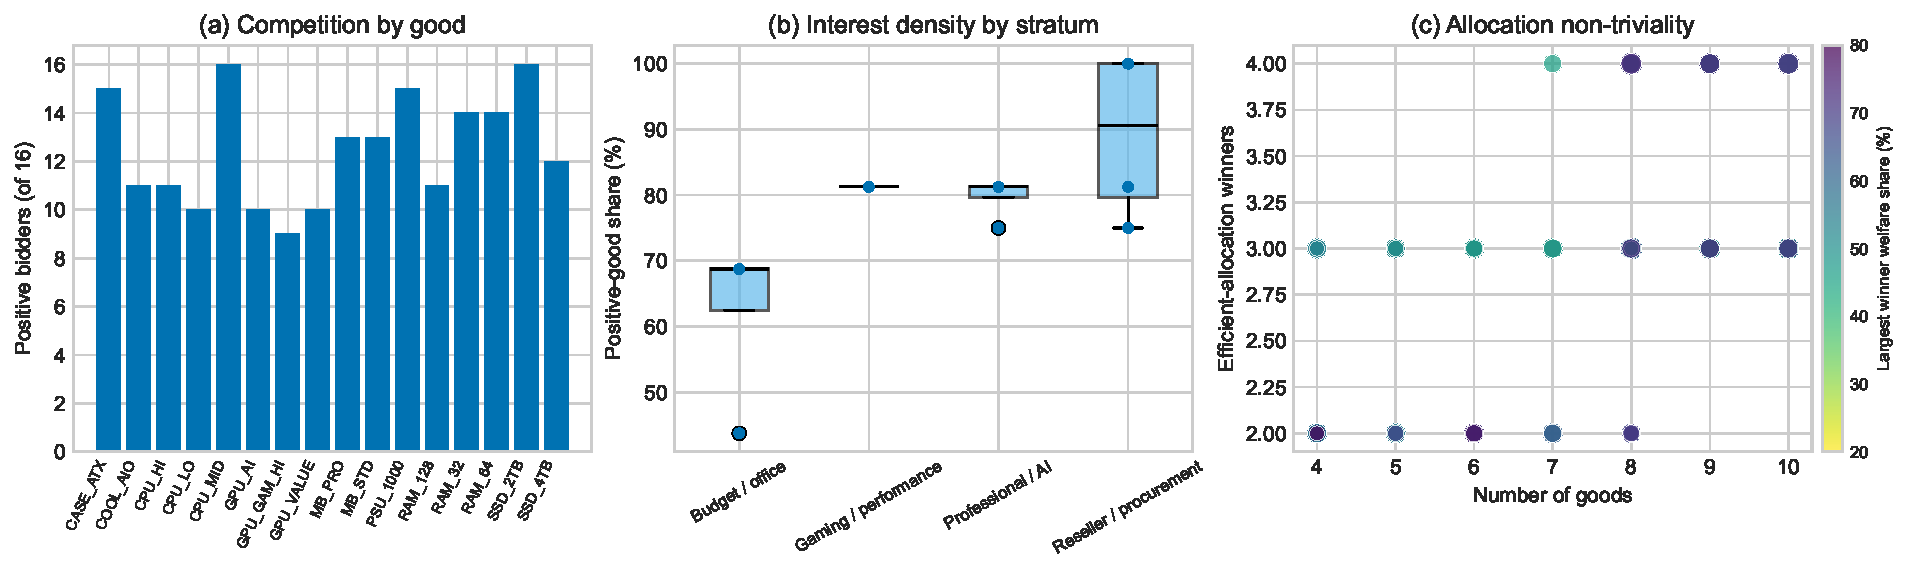
\includegraphics[width=\linewidth]{outputs/final/analytic_package_v3/figures/environment_structure.pdf}
    \caption{Structure of the generated experimental environment. Panel (a)
    reports positive bidders per master-population good; panel (b) reports
    bidder interest density by stratum; panel (c) reports full-information
    winner counts across accepted cells, with colour indicating the largest
    winner's welfare share and marker size indicating bidder count.}
    \label{fig:environment-structure}
\end{figure}

\subsection{Provisional-Value Calibration}

The out-of-domain calibration selects a uniform scale of 1.4758. Across nine
held-out synthetic environments, mean normalised payment error falls from
0.289 without calibration to 0.233 with calibration, a 19.5\% relative
reduction; seven of nine held-out cases improve. The scale is therefore used
for all initial provisional bids in the final PC-component experiments.

\subsection{Interest-Map Support Reduction}

Figure~\ref{fig:interest-support} compares the full non-empty powerset with
final candidate support. Final support excludes every bundle containing an
inferred-uninterested good and every bundle containing multiple members of an
evidence-grounded \texttt{choose\_one} group. Across all 95 cases it is 55.5\%
smaller than the full-support baseline. With eight bidders and ten goods,
support falls from 8,184 bidder--bundle valuations to 2,619.2 candidates, a
68.0\% reduction. At the \(8\times8\) anchor, it falls from 2,040 to 757.6
on average.

\begin{figure}[htbp]
    \centering
    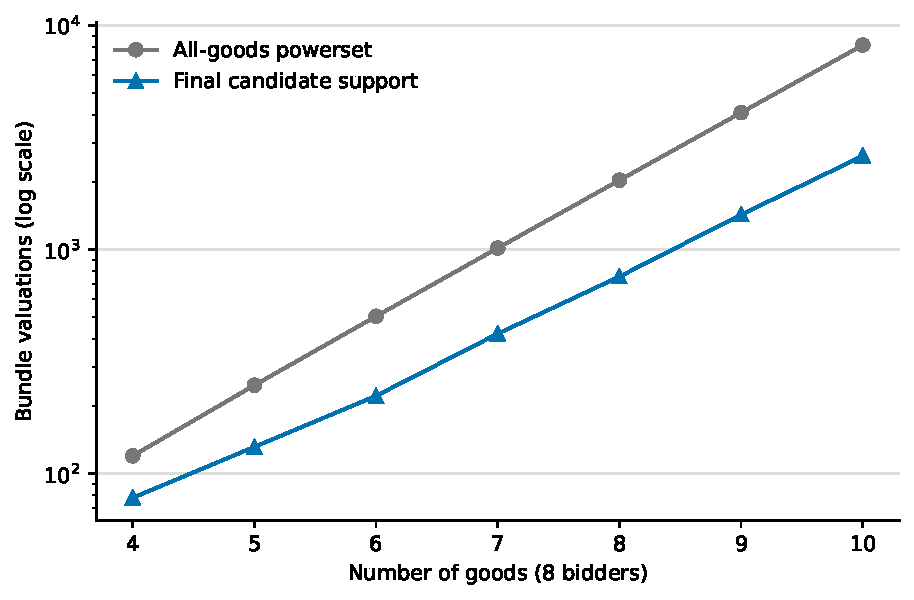
\includegraphics[width=0.76\linewidth]{outputs/final/analytic_package_v3/figures/interest_map_candidate_support.pdf}
    \caption{Auction-level candidate-support size with eight bidders as the
    number of goods varies. Points are five-seed means; the vertical axis is
    logarithmic. The full baseline is \(8(2^{|G|}-1)\).}
    \label{fig:interest-support}
\end{figure}

This reduction changes the practical level of the communication problem but
does not remove exponential worst-case growth. Its interpretation is also
deliberately narrow. The opening disclosures are validated against hidden
profiles before interest-map inference, so high reconstruction accuracy is a
pipeline check on reconstruction from validated disclosure, not evidence of
unrestricted preference recovery from arbitrary language.

\subsection{Event-Policy Ablations}
\label{sec:policy-ablation}

Policy selection uses five-seed \(8\times8\) ablations and precedes the
95-case evaluation. In the sealed study, incumbent verification alone
achieves 92.2\% mean efficiency with 11.2 queries. Adding winner-removal
counterfactuals raises efficiency to 95.6\% with 19.0 queries; adding
scarcity fallbacks reaches 97.8\% with 22.4; and the full \emph{adaptive
competitive-frontier refinement} (ACFR) policy, including large-correction
follow-up, reaches 99.1\% with 26.2. Removing incumbent verification produces
the largest degradation, to 89.4\%.

The clock ablation holds the top-three, \$50-step price path fixed and varies
only terminal events. PV-only supplementary allocation achieves 88.1\% with
no exact query. A single revealed-witness treatment reaches 90.2\% with three
queries; winner closure reaches 92.2\% with 11.2; and the selected
revealed-winner sandwich reaches 95.7\% with 13.4. Full frontier closure is
slightly less efficient at 95.2\% while using 21.4 queries. The sandwich is
therefore the best observed efficiency--query trade-off among the tested
policies, rather than a claim that adding events is monotonically beneficial.

A leave-one-composition-seed-out stability check provides a limited guard
against selection by one favourable ordering. Maximising mean efficiency on
four seeds selects ACFR in all five sealed folds, with a tie against the
policy without scarcity in one fold; ACFR's held-out mean is 99.1\%. The
revealed-winner sandwich is selected in all five clock folds and retains
95.7\% held-out mean efficiency. This supports stability across the available
compositions, but it is not validation on a newly generated population.

\begin{figure}[htbp]
    \centering
    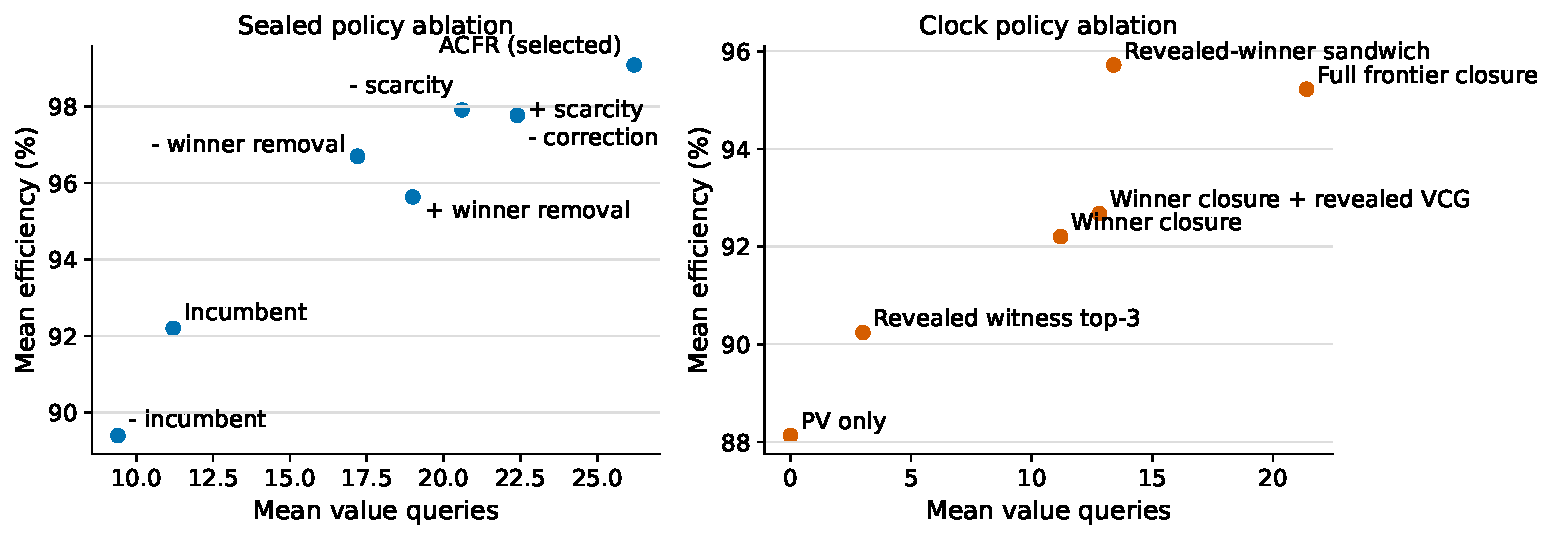
\includegraphics[width=\linewidth]{outputs/final/analytic_package_v3/figures/event_policy_ablation.pdf}
    \caption{Five-seed \(8\times8\) event-policy ablations. The selected
    policies are adaptive competitive-frontier refinement for sealed and the
    revealed-winner sandwich for clock.}
    \label{fig:policy-ablation}
\end{figure}

\subsection{Full-Suite Overview}

Table~\ref{tab:final-summary} gives the main paired results. The calibrated
initial bids achieve 86.4\% mean efficiency. Sealed elicitation raises this
to 94.8\%, a paired gain of 8.4 percentage points (seed-clustered 95\% CI
3.9--12.9), and improves 78 of 95 cases. Clock elicitation raises mean
efficiency to 92.8\%, a 6.5-point gain (95\% CI 1.3--11.6), and improves 68
cases. Selective exact correction is non-monotonic: sealed worsens two cases
and clock worsens 12 because the WDP continues to compare corrected atoms
with remaining provisional atoms.

\begin{table}[htbp]
\centering
\small
\caption{Final allocation and communication results over 95 matched cases.
Efficiency intervals use five seed-level means. Better/same/worse compares
each elicited mechanism with its common initial provisional allocation.}
\label{tab:final-summary}
\begin{tabular}{@{}lrrrrrr@{}}
\toprule
Arm & Mean eff. & Median & 95\% CI & \(\eta\geq95\%\) & Exact & Mean VQs \\
\midrule
Initial PV & 86.4\% & 88.2\% & 82.3--90.5\% & 19 & 7 & 0.0 \\
Sealed & 94.8\% & 97.8\% & 93.7--95.8\% & 57 & 23 & 21.8 \\
Clock & 92.8\% & 95.0\% & 88.8--96.8\% & 48 & 15 & 12.3 \\
\bottomrule
\end{tabular}
\end{table}

Figure~\ref{fig:efficiency-scaling} shows all three scalability paths. Mean
sealed efficiency is 95.0\% when bidders vary at eight goods, 94.5\% when
goods vary at eight bidders, and 96.0\% along the joint path, with the common
anchor included in each visual series. Clock gives 94.4\%, 92.4\%, and
92.5\%, respectively. The curves are non-monotonic because successive cells
are nested changes in composition rather than iid draws, but they show no
collapse in average efficiency through the \(10\times10\) endpoint.

\begin{figure}[htbp]
    \centering
    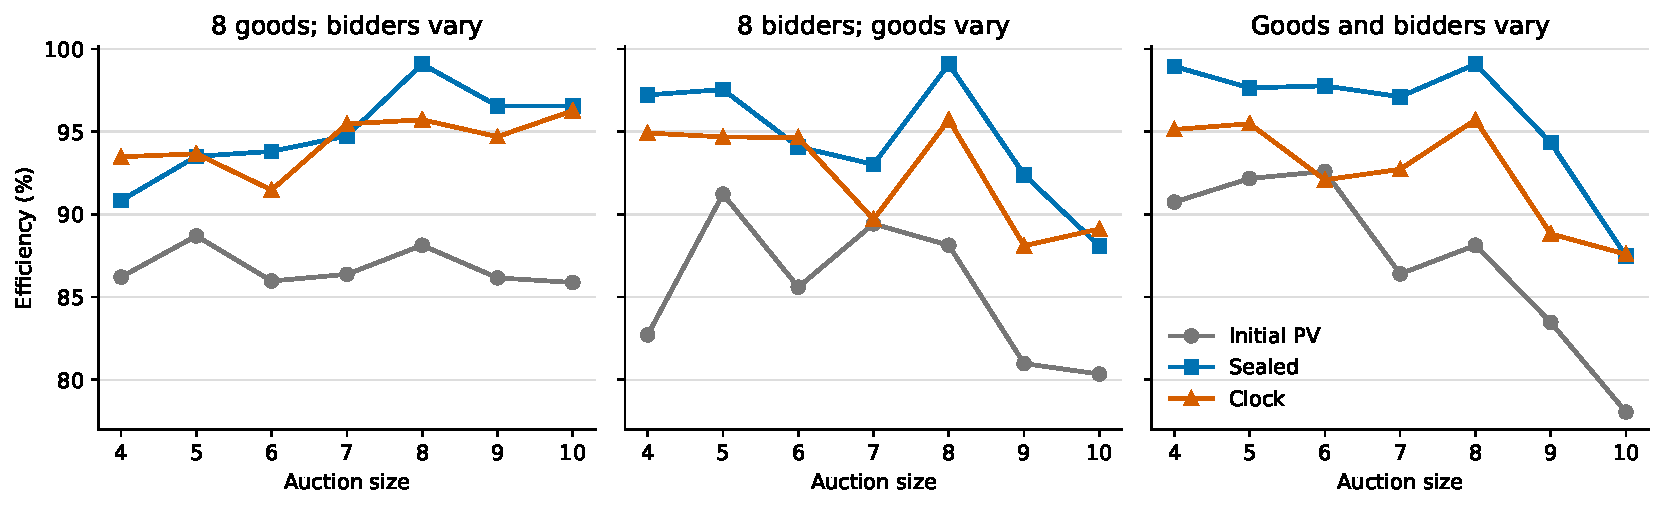
\includegraphics[width=\linewidth]{outputs/final/analytic_package_v3/figures/efficiency_scaling.pdf}
    \caption{True allocation efficiency across the bidder, goods, and joint
    scalability paths. Lines show cell means over five seeds and points show
    seed-level observations. The \(8\times8\) anchor appears in each panel.}
    \label{fig:efficiency-scaling}
\end{figure}

The final event policies produce a clear query trade-off.
Figure~\ref{fig:query-scaling} shows 21.8 exact VQs per sealed case and 12.3
per clock case. Clock uses 9.6 fewer queries on average (seed-clustered 95\%
CI 7.4--11.7 fewer) and is less query-intensive in 86 of 95 paired cases.
This is a consequence of the final clock redesign: price discovery itself
makes no exact query, and only revealed terminal winners and VCG witnesses
are eligible for verification. The sealed mechanism searches its allocation
and counterfactual frontier during every elicitation round.

\begin{figure}[htbp]
    \centering
    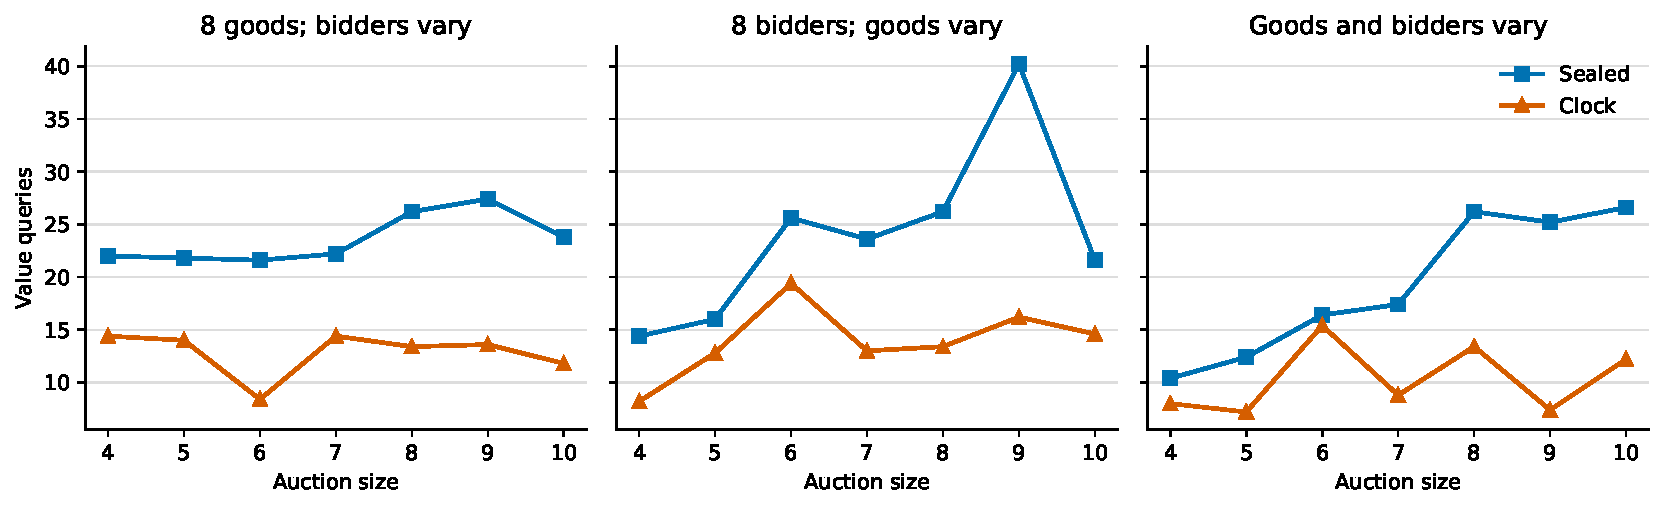
\includegraphics[width=\linewidth]{outputs/final/analytic_package_v3/figures/value_queries_scaling.pdf}
    \caption{Deterministic exact value queries across the final scalability
    suite. Offline disclosure, interest-map, and provisional-valuation calls
    are excluded.}
    \label{fig:query-scaling}
\end{figure}

All 95 clock auctions clear through no excess demand. The median clock lasts
30 rounds, the mean 33.6, and the maximum 84. Seventeen cases require more
than 50 rounds, confirming that the frozen 500-round value is a safeguard
rather than a binding termination rule. Sealed elicitation stops after a
median of five and a maximum of 29 refinement rounds, below its 40-round
safeguard.

\subsection{Sealed Outcomes and Event Path}

The final suite records allocation incidence and reported-VCG-witness
incidence for every exact query. In sealed ACFR, allocated bundles account for
742 queries and winner-removal counterfactuals for 683; 30.5\% and 31.3\%,
respectively, appear in the final reported VCG witness set. Large-correction
follow-ups account for 288 queries with a 27.1\% witness hit rate. Scarcity
fallbacks account for 361 queries and have a lower 11.6\% direct witness rate.
That lower rate does not establish zero causal value: an exact fallback can
alter an intermediate allocation and expose a later winner or
counterfactual.

Across all sizes, ACFR reaches 94.8\% mean efficiency with 21.8 exact queries,
improving 78 of 95 initial allocations. Its median of five refinement rounds
reflects repeated WDP feedback rather than a fixed query schedule. In the
seed-zero four-good, eight-bidder example, incumbent and counterfactual events
raise efficiency from 45.7\% to 96.6\% in five rounds and 15 queries. This
illustrates the intended sealed logic: verify the reported winner, expose its
nearest allocation competitors, and re-optimise after correction.

\subsection{Clock Outcomes and Event Path}

In the clock mechanism, winner closure accounts for 754 queries with a 29.7\%
reported-witness hit rate. The staged revealed-witness phase accounts for 125
queries with a 40.8\% hit rate, while the frozen single-pass revealed-witness
stage is the most targeted: 57.5\% of its 287 queries enter the final reported
witness set. These diagnostics show how the clock's demand path restricts
verification without eliminating payment-relevant bundles.

The clock reaches 92.8\% mean efficiency with 12.3 exact queries and improves
68 of 95 initial allocations. Every price path clears through zero excess
demand before terminal verification. Its lower query count follows directly
from price-path eligibility: an unobserved losing atom cannot enter the
revealed-witness frontier. The trade-off is narrower corrective coverage and
12 cases in which terminal correction lowers efficiency relative to the
initial supplementary allocation.

\begin{figure}[htbp]
    \centering
    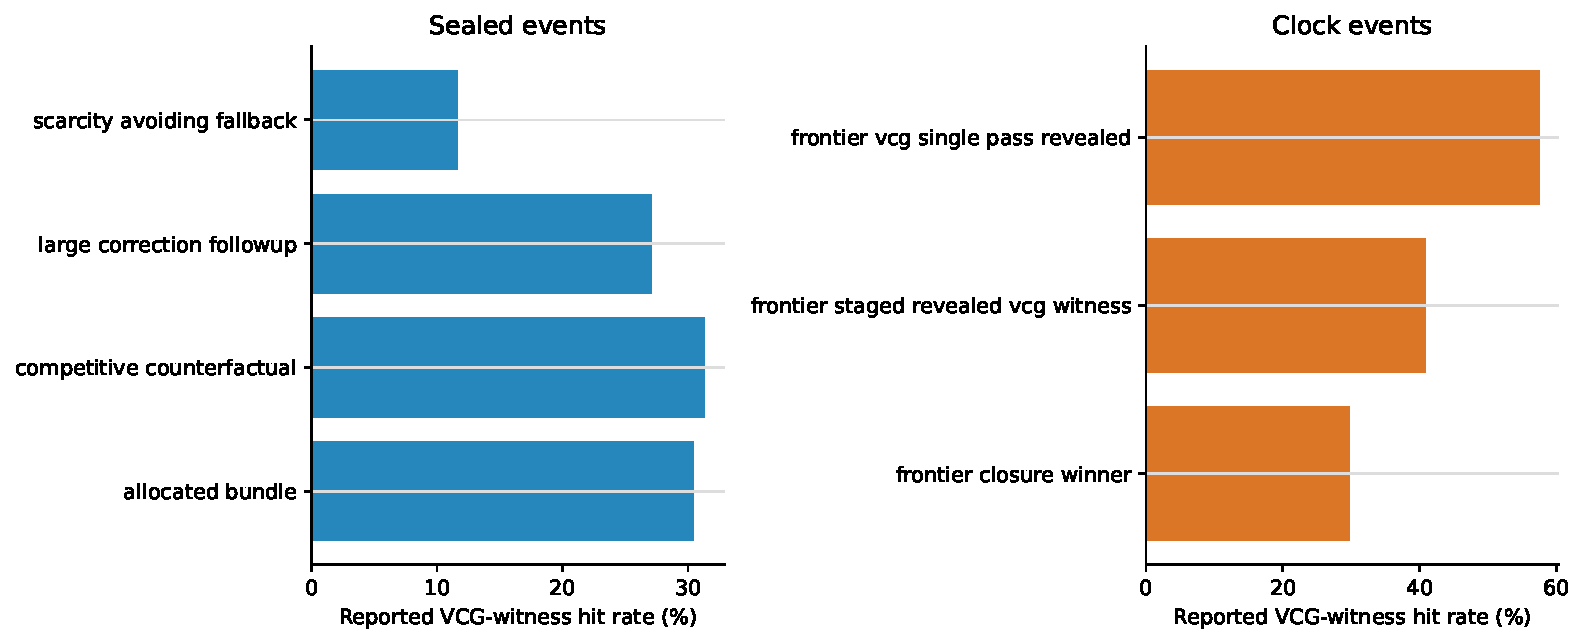
\includegraphics[width=\linewidth]{outputs/final/analytic_package_v3/figures/event_usefulness.pdf}
    \caption{Reported VCG-witness incidence by event type over the final
    95-case suites. Incidence is descriptive rather than a causal ablation.}
    \label{fig:event-usefulness}
\end{figure}

Figure~\ref{fig:illustrative-path} contrasts the successful sealed path above
with a clock failure. The seed-zero \(6\times6\) clock case begins with a fully
efficient supplementary allocation but terminal corrections select an
allocation at 76.2\% efficiency after 13 queries. Exact local corrections
need not improve the global allocation while other atoms remain provisional.

\begin{figure}[htbp]
    \centering
    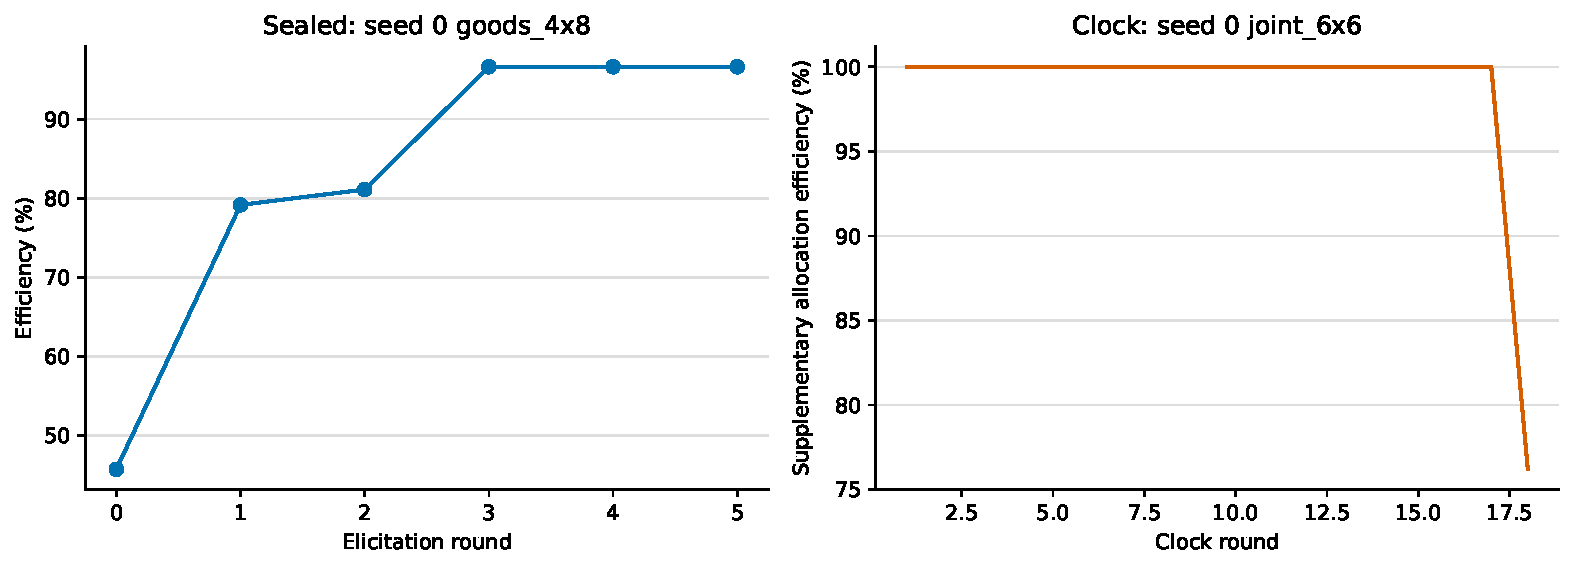
\includegraphics[width=\linewidth]{outputs/final/analytic_package_v3/figures/illustrative_trajectories.pdf}
    \caption{Illustrative final-suite trajectories: the largest sealed
    efficiency gain (left) and largest clock terminal welfare reduction
    (right). These are diagnostic examples, not representative averages.}
    \label{fig:illustrative-path}
\end{figure}

\subsection{Cross-Mechanism Comparison and the Payment-Counterfactual Gap}

Sealed exceeds clock efficiency by 1.9 percentage points on average. Clock
is higher in 21 cases, the mechanisms are equal in 22, and sealed is higher
in 52. However, the seed-clustered 95\% interval for clock minus sealed is
--5.1 to 1.2 points, so five composition seeds do not resolve a population
difference in efficiency. Figure~\ref{fig:cross-mechanism} shows both the
concentration near equality and several mechanism-specific failures.

\begin{figure}[htbp]
    \centering
    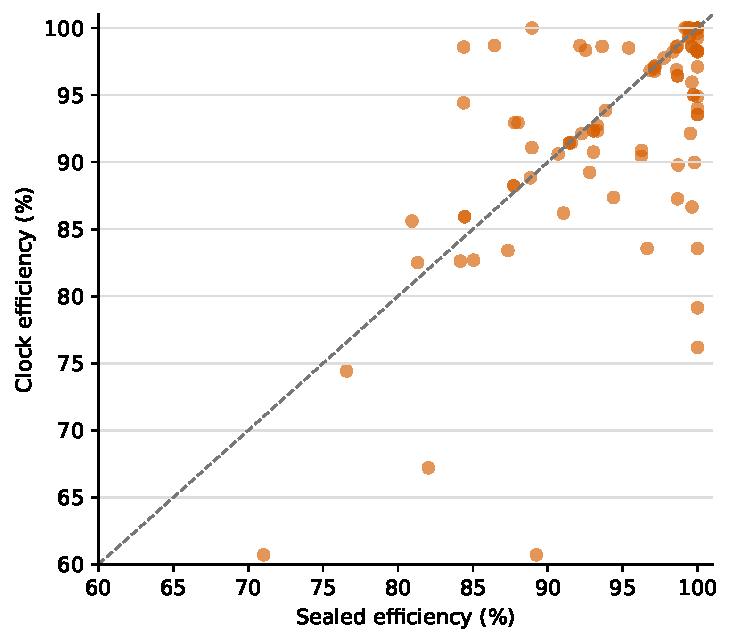
\includegraphics[width=0.62\linewidth]{outputs/final/analytic_package_v3/figures/cross_mechanism_efficiency.pdf}
    \caption{Paired sealed and clock efficiency under the same frozen initial
    proxy state. The dashed line denotes equal efficiency.}
    \label{fig:cross-mechanism}
\end{figure}

Payment reconstruction is a separate and more demanding information problem,
as Table~\ref{tab:allocation-payment-information} makes explicit. An efficient
allocation can be supported by accurate values for a small set of winning and
displacing bundles. VCG additionally requires a correctly reported
bidder-removal optimum for every winner.

\begin{table}[htbp]
\centering
\small
\caption{Different information requirements for allocation and VCG pricing.}
\label{tab:allocation-payment-information}
\begin{tabular}{@{}p{0.19\linewidth}p{0.34\linewidth}p{0.36\linewidth}@{}}
\toprule
Outcome & Required reported information & Sparse-elicitation failure \\
\midrule
Efficient allocation & Values sufficient to rank feasible allocations near \(a^*\) & Winning or close competing bundle is omitted or misranked \\
Winner \(i\)'s VCG payment & Allocation information plus accurate \(W^*_{-i}\) & Bidder-removal witness remains provisional, omitted, or unrevealed \\
\bottomrule
\end{tabular}
\end{table}

Empirically, payment reconstruction remains materially weaker than allocation recovery.
Mean absolute per-winner payment error, normalised by optimum welfare, is
32.1\% for sealed and 36.5\% for clock. The corresponding absolute revenue
errors are 12.0\% and 13.4\%. Paired payment-error and revenue-error
differences both have seed-clustered intervals crossing zero. Figure
\ref{fig:payment-scaling} shows that high allocation efficiency does not
force reported-space VCG payments to approach the oracle payments: each
winner's payment also depends on welfare in a bidder-removal allocation whose
support may remain provisional or unrevealed.

\begin{figure}[htbp]
    \centering
    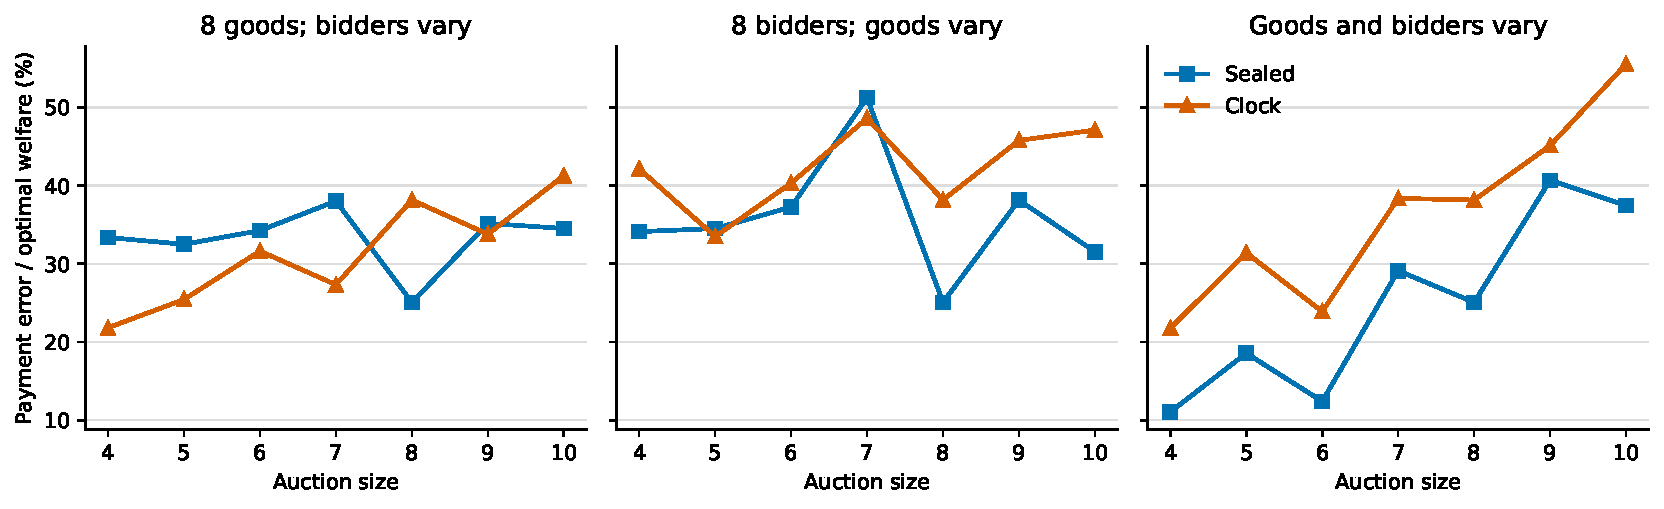
\includegraphics[width=\linewidth]{outputs/final/analytic_package_v3/figures/payment_error_scaling.pdf}
    \caption{Absolute reported-space VCG payment error normalised by
    full-information optimum welfare. Lower is better.}
    \label{fig:payment-scaling}
\end{figure}

\section{Discussion}

\subsection{Support Selection and Provisional Scoring}

The interest map and provisional valuation solve different problems.
Interest-map inference is a support-selection decision: excluded items and
evidence-grounded acquisition modes determine which bundles can enter the
initial bid. Provisional valuation is a scoring decision conditional on that
support. A candidate omitted by the interest map cannot be recovered merely
by improving the PV prompt. Conversely, a broad support does not guarantee a
good allocation if allocation-relevant bundles are badly ranked.

This decomposition is useful both scientifically and operationally. Exact
values on interest-map support measure the best outcome available after
support filtering. Comparing that benchmark with proxy PV identifies scoring
loss. Comparing oracle and inferred candidate sets identifies exclusion and
substitute-mode loss. It also prevents interest-map performance from being
judged only through the final auction outcome, where several errors interact.

\subsection{Mechanisms as Elicitation Environments}

Sealed and clock auctions begin from the same frozen proxy state but expose
different reasons to revisit a bundle. Competitive sealed feedback searches
the reported allocation frontier directly throughout its iterative phase.
The final clock policy instead uses the price path as a relevance filter: it
first discovers demand without exact queries, then verifies newly exposed
winners and bidder-removal witnesses only when those witnesses were revealed
on the clock path. The event interface makes these differences explicit
without embedding LLM orchestration inside the auction mechanism.

The ablations show that more querying is not automatically better. Full
clock-frontier closure uses eight more queries than the selected sandwich yet
has slightly lower mean efficiency. Direct event ``hits'' must nevertheless
be interpreted cautiously. A queried
bundle need not appear in the final or full-information allocation to be
causally useful. Correcting it can change an intermediate WDP allocation,
which exposes another winner or counterfactual bundle. Event evaluation
therefore combines direct final-allocation incidence with trajectory and
ablation evidence.

\subsection{Non-Monotonic Refinement}

Refinement is not guaranteed to improve true welfare monotonically. The WDP
optimises a mixture of exact queried values and uncorrected provisional
values. Correcting one bundle can therefore move the reported optimum to an
allocation with lower hidden welfare, even though the individual correction
is exact. This is a central feature of selective elicitation rather than
necessarily an implementation defect. Useful query policies must be both
value-correcting and allocation-relevant, and reported trajectories should
not be assumed to converge monotonically.

\subsection{Preparation Cost and Person-Side Query Cost}

The implementation separates person-model disclosures, verification,
interest-map inference, PV chunks, value queries, and demand queries. This
matters because their costs have different interpretations. Person and proxy
tokens are one-off offline preparation costs attached to frozen packs.
Mechanism-triggered VQs are person-side preference queries, but in the
principal experiment they are deterministic and consume no LLM tokens.
Mechanism runtime therefore scales in WDP solves, clock rounds, and exact
queries rather than hosted-model calls.

Interest-map filtering reduces the candidate powerset by 55.5\% on average,
but support generation still grows rapidly for broad-interest bidders. PV
chunking improves structured-output reliability; it does not change the
underlying number of candidate bundles that must be scored. Candidate count
and preparation cost must therefore remain conceptually separate from
auction-stage exact-query counts. The reported mechanism comparison concerns
the latter because all offline inference is shared and amortisable.

\subsection{Allocation and Payment Accuracy}

Sparse elicitation places different information demands on allocation and
VCG pricing. Efficient allocation requires enough information to rank
feasible outcomes near the optimum. Accurate VCG payments additionally
require winner-removal welfare. A large revenue difference at high
allocation efficiency is therefore informative rather than contradictory:
it indicates that the allocation frontier was learned more accurately than
the payment counterfactual frontier. VCG-witness logging makes this
distinction observable, but the residual 32--36\% normalised payment error
shows that the selected sparse policies do not fully close bidder-removal
support.

\section{Limitations}

Four limitations most directly bound the paper's claims:
\begin{enumerate}[leftmargin=*]
    \item \textbf{One domain and one generated population.} The five
    composition seeds are nested samples from one validated 16-by-16 master
    population, not five independently generated populations. Statistical
    intervals therefore describe composition sensitivity within this
    population.
    \item \textbf{No strategic behaviour.} Provisional estimates and exact
    refinements are treated as reports to be corrected, without bid shading,
    manipulation, or equilibrium analysis. The mechanisms are experimental
    elicitation environments rather than deployment-ready auction designs.
    \item \textbf{No human-subject evidence.} The architecture reduces formal
    reporting and presents a natural-language interface, but it does not
    establish that real bidders experience lower cognitive burden or can
    answer repeated exact value queries consistently.
    \item \textbf{Policy selection within the same population.} The
    \(8\times8\) ablations and 95-case evaluation share the master population.
    Leave-one-seed-out stability helps only across compositions; it does not
    establish transfer to a new domain or independently generated population.
\end{enumerate}

Additional modelling limitations remain. Population constraints and the
deterministic valuation formula encode judgement about complements,
substitutes, budgets, caps, and saturation. The fixed model assignment,
validated disclosures, and closed-world interest map may overstate inference
reliability relative to incomplete or strategic human language. Candidate
support is frozen rather than revised online. The CCA-inspired clock omits
activity rules, a full supplementary-bidding phase, optimised increments, and
core-selecting payments. The current environment also assumes unit-supply
indivisible goods. Model-role robustness, other mechanisms such as CECA, and
independently generated domains remain future validation rather than evidence
claimed here.

\section{Extensions}

Natural extensions include:
\begin{itemize}[leftmargin=*]
    \item dynamic interest-map updates after mechanism feedback;
    \item uncertainty-aware event priority based on pivotality and confidence;
    \item a bounded post-allocation payment-counterfactual audit;
    \item demand-query and noisy human-response robustness treatments;
    \item interval-valued or uncertainty-calibrated provisional valuations;
    \item CCA-lite activity rules and core-selecting payments;
    \item strategic proxy policies;
    \item independently generated populations, domains, and multi-model role robustness;
    \item human-subject validation of the person-simulator assumptions;
    \item CECA-style satisfaction and counterexample event adapters.
\end{itemize}

\section{Conclusion}

This paper develops a reproducible framework for scalable preference
elicitation with LLM proxy bidders. A constrained generation-and-validation
pipeline supplies structured private benchmark environments. A
language-to-bid pipeline separates candidate selection through an interest
map from candidate scoring through provisional valuations. A modular event
interface then embeds the same frozen proxy state in iterative sealed and
ascending clock auctions.

The separation between support, scoring, and refinement is central. It makes
candidate omission distinguishable from provisional misvaluation and makes
mechanism feedback comparable without repeated LLM sampling. The
closed-world interest map provides scalability, while evidence-grounded
acquisition modes protect multi-use bidders from overly aggressive
substitute filtering. Frozen replay and deterministic value queries isolate
the economic query path from hosted-model variability.

The framework does not remove the exponential communication problem for
general combinatorial values. Instead, it provides a controlled empirical
method for studying where information is discarded, how initial bids are
formed, and which allocation- or price-derived events recover
decision-relevant values. This makes the interaction between language
inference and auction design observable, reproducible, and amenable to
ablation.

In the final five-composition-seed evaluation, interest maps reduce candidate support by
55.5\% relative to full powersets. Calibrated provisional bids achieve 86.4\%
mean efficiency; sealed and clock elicitation raise this to 94.8\% and 92.8\%
with 21.8 and 12.3 exact value queries, respectively. The selected clock
policy preserves genuine ascending-price discovery and clears naturally in
all 95 cases, while its revealed-demand restriction substantially reduces
query volume. Neither policy reconstructs VCG payments as successfully as it
reconstructs allocations, identifying sparse payment-counterfactual closure
as the most important remaining mechanism-design problem.

\appendix
\section{Reproducibility and Additional Specification}
\label{app:reproducibility}

\subsection{Frozen Model Roles and Information Boundaries}

The accepted master population was generated by OpenAI
\texttt{gpt-5.6-sol}. Frozen opening answers and their independent verifier
calls also use \texttt{gpt-5.6-sol}. Interest maps and provisional valuations
use Google \texttt{gemini-3.6-flash}. The bidder proxy receives only the
public catalogue and accepted opening exchange; it never receives latent
profiles or complete valuation tables. All auction-stage exact answers are
deterministic lookups and therefore use no model provider.

The five composition seeds \(0,\ldots,4\) instantiate distinct nested goods
and bidder orderings from the same master population. Each goods-specific
master elicitation pack is projected to smaller bidder sets, ensuring that
changing the number of rivals does not regenerate a bidder's opening exchange
or provisional values.

\subsection{Frozen Preparation and Mechanism Parameters}

\begin{table}[htbp]
\centering
\small
\caption{Principal frozen parameters. Zero query caps denote disabled caps.}
\label{tab:frozen-parameters}
\begin{tabular}{@{}p{0.31\linewidth}p{0.23\linewidth}p{0.34\linewidth}@{}}
\toprule
Component & Setting & Value \\
\midrule
Opening interaction & Question policy & Canonical, one accepted answer \\
Interest map & World assumption / failure & Closed world / fail closed \\
Candidate support & Maximum bundles & Uncapped \\
Provisional valuation & Chunk / failure & 64 bundles / fail closed \\
Parsing & Additional retries & 2 \\
Calibration & Family / scale / size factor & Uniform / 1.4758 / 1.0 \\
Sealed & Events & Incumbent, winner removal, scarcity, correction follow-up \\
Sealed & Stop / safeguard & No new refinements / 40 rounds \\
Sealed & Correction / scarcity threshold & 25\% / 60\% of incumbent report \\
Clock & Demand / price increment & Top three / \$50 \\
Clock & Stop / safeguard & No excess demand / 500 rounds \\
Clock & Terminal policy & Single-pass revealed witness and staged winner/witness closure \\
Queries & Per-bidder / global cap & 0 / 0 \\
Queries & Exact response mode & Deterministic hidden-value lookup \\
\bottomrule
\end{tabular}
\end{table}

Structured-output parsing is fail closed in the principal preparation. A
failed interest map or provisional-value chunk is retried with diagnostic
context and then aborts rather than silently expanding to all goods or
replacing the treatment with mass exact queries. Successful model responses
are committed independently to a read-write SQLite cache keyed by the rendered
prompt and response-relevant settings. Frozen packs record raw and parsed
responses, model role, token counts, latency, cache status, candidate support,
and configuration hashes.

\subsection{Frozen Artifacts and Offline Reconstruction}

The experiment is anchored by
\texttt{outputs/final/final\_experiment\_v3.json}, which records scenario and
pack hashes, calibration provenance, event policy, mechanism parameters, and
all 95 pack paths. Raw sealed and clock outputs are stored under
\texttt{outputs/final/scalability\_v2} and
\texttt{outputs/final/clock\_sandwich\_scalability\_v3}. The final analysis
is reconstructed without LLM calls by:

\begin{verbatim}
./venv/bin/python scripts/build_final_analytic_package.py \
  --spec outputs/final/final_experiment_v3.json \
  --sealed-dir outputs/final/scalability_v2 \
  --clock-dir outputs/final/clock_sandwich_scalability_v3 \
  --interest-map-dir outputs/interest_map_analysis \
  --sealed-ablation outputs/final/event_policy_8x8 \
  --clock-ablation \
    outputs/final/clock_focused_closure_ablation_pc_8x8_calibrated \
  --output-dir outputs/final/analytic_package_v3
\end{verbatim}

Generated-environment tables and Figure~\ref{fig:environment-structure} are
reconstructed from the accepted population and its validation report:

\begin{verbatim}
./venv/bin/python scripts/analyze_generated_environment.py \
  --scenario-spec \
    scenarios/pc_build_v3/pc_build_population_16x16.json \
  --validation-report \
    scenarios/pc_build_v3/pc_build_population_16x16.validation.json \
  --output-dir outputs/final/analytic_package_v3
\end{verbatim}

The analytic package contains case-level inputs, seed-clustered summaries,
event and VCG-witness diagnostics, calibration evidence, selected trajectories,
environment tables, and both PDF and PNG figures. Rebuilding these outputs
does not mutate the frozen scenario, elicitation packs, or auction runs.

\bibliographystyle{plainnat}
\bibliography{references}

\end{document}
